
\chapter{Introduction}
\label{chap:introduction}

\section{Steps by steps to R}

\begin{enumerate}
  \item If you haven't installed R, read Sect.\ref{sec:R-install}
  
  \item Once you open R GUI: a prompt will show 
\begin{verbatim}
>
\end{verbatim}
where we can type in commands. 

NOTE: Of course, we can also run from a script file


  \item Type in the first few commands: execute a function

In R, in order to be executed, a function always needs to be written with parentheses, even if there is nothing within them
\begin{verbatim}
> ls()
\end{verbatim}

If one just types the name of a function without parentheses, R will display the content of the function.

  \item To get help (Sect.\ref{sec:getting-helps}), at any time, from the
  prompt, type
\begin{verbatim}
help.start()
\end{verbatim}
  
  \item R is a language which is both a functional language
  (Sect.\ref{sec:R-functional}) and an object-oriented language
  (Sect.\ref{sec:R-object-oriented})
  
variables, data, functions, results, etc, are stored in the active memory of the
computer in the form of {\bf objects} which have a name.
Functions  are themselves objects. We access to an object via its name. We
manipulate an object by calling operators (arithmetic, logical, comparison, ...)
and functions.


  \item Type in the first few commands: assigmnent to create a named-object
  
While R is running, variables, data, functions, results, etc, are stored in the
active memory of the computer in the form of objects which have a name.

  

R is an interpreted language, not a compiled one, meaning that all commands
typed on the key- board are directly executed without requiring to build a
complete program like in most computer languages (C, Fortran, Pascal, \ldots)

  \item 

\end{enumerate}


\section{History of R}
\label{sec:history-r}

S is a statistical programming language built to run on GCOS operating
system (target to mainframe computers
only)\footnote{\url{http://cm.bell-labs.com/cm/ms/departments/sia/S/history.html}}.
The aim of the language, ``to turn ideas into software, quickly and
faithfully'' as expressed by John Chambers (who invented S).

S is a {\it functional language}, and methods in the language are
function-based, not class-based.  There are two implementation of S:
the freeware, R, and the commercial software, S-PLUS.

R is open-source software which implements the S programming language
using C and FORTRAN, with some modification, i.e. its semantics are
derived from Scheme programming language. Scheme is a multi-paradigm
programming language derived from LISP. 

\begin{mdframed}

NOTE: Here is the list of different programming paradigms:

\begin{itemize}
\item dataflow (e.g. spreadsheets like Excel) 
\item visual programming language (e.g. Simulink)
\item functional programming language (e.g. Perl)
\item procedural programming language (e.g. Pascal, C)
\item object-oriented (OO) \~{} parallel computing (e.g. C++, Fortran 2003,
  Java, C\#)
\item constraint programming (e.g. Prolog)
\item declarative programming (e.g. HTML)
\end{itemize}
\end{mdframed}

\textcolor{blue}{So, the R language is a two-paradigm programming
  language}.
Beside as a functional language (Sect.\ref{sec:R-functional}), R now supports
class-based method (Object-Oriented) - Sect.\ref{sec:R-object-oriented}.

Current R is compatible with version 4 of S, S4, which provides
advance OO features since classes of S4 differ markedly from S3
classes. Version 4 has been developed since 1998 (add formal
class-method model, connections, large objects), 1999 (interfaces to
Java, Corba).


Wiki: ``{\it Up to this date, much of the statistical computing was done by
directly calling FORTRAN subroutines; however, S was designed to offer
an alternate and more interactive approach}''


\textcolor{blue}{One of the most important things in R to remember is
that every thing is an object, even for functions and expressions (a
value, a variable, a vector or matrix, a dataset)}.
An object is determined by 2 criteria:

\begin{itemize}
\item MODE\label{mode}:
  {\it logical, complex, factor, numeric, character, list,
    raw, any},
  and {\it function}. The MODE of an object is automatically
  determined by the types of things stored in it.

\item CLASS\label{class}: [vector] matrix, array, data.frame, and hundreds of
  special classes created by specific functions. The CLASS of an
  object is set by default depending on how it was created. However,
  it can be changed explicitly, since it is a way that determines how
  functions deal with the object. Depending on the object's CLASS, the
  object will behave differently in different functions.

\end{itemize} 

A collection (database) of objects is tended to be called
{\it libraries} if the objects are mainly functions. In R, for
functions, there is no 'pass by reference' parameters, only 'pass by
value'.  'A graphics are written out and are not stored as
objects'. Thus, the only way to save a figure is to open a connection
to the device (files, printer, ...)  before do any plotting
operation. For example, save the figure to a postscript format:
\begin{lstlisting}
postscript("filename.eps")
plot(x,y) 
dev.off()
\end{lstlisting}


\subsection{functional aspect of R}
\label{sec:R-functional}


Variables, data, functions, results, etc, are stored in the active memory of the
computer in the form of {\bf objects} which have a name. A function is also an
object in R.

Executing a function needs (1) arguments; and (2) options (which are arguments
with default values), and this returns a result.
\begin{itemize}

  \item The arguments can be objects (“data”, formulae, expressions, . . . ),

An R function may require no argument: either all arguments are defined by
default (and their values can be modified with the options), or no argument has
been defined in the function.

\end{itemize}

The basic of understanding a functional languge is to know how an assignment works

\subsection{-- quotes in R: single, double quotes or backtick}


Three types of quotes are part of the syntax of R: single and double quotation
marks and the backtick (or back quote, `)

\url{https://stat.ethz.ch/R-manual/R-devel/library/base/html/Quotes.html}

\subsection{-- creating the first object using assignment in R}

As 'x' is a name, assigning a value to it can be done via different ways:
two of them have leftwards and rightwards forms.
The name x can be a name or an expression defining a part of an object to be
replaced (e.g., \verb!z[[1]]!)

\begin{verbatim}

x <- value
x <<- value

value -> x
value ->> x

x = value
\end{verbatim}

EXPLAIN:
\begin{enumerate}
  \item  The operator \verb!<-! can be used anywhere, 
  
  \item whereas the operator \verb!! is only allowed at the top level 
  (e.g., in the complete expression typed at the command prompt) or as one of the subexpressions in a braced list of expressions.
  
  \item The operators \verb!<<-! and \verb!->>! are normally only used in
  functions, and cause a search to be made through parent environments for an
  existing definition of the variable being assigned.
  
  If such a variable is found (and its binding is not locked) then its value is
  redefined, otherwise assignment takes place in the global environment.
  
  \item 
  
\end{enumerate}

\subsection{-- how to manage objects in memory}



\subsection{object-oriented aspect of R}
\label{sec:R-object-oriented}

Designers of R language try to combine aspects of {\it functional} and {\it
object-oriented} (i.e., method-centered)
approaches'\footnote{\url{http://cm.bell-labs.com/cm/ms/departments/sia/S/history.html
}}.

\begin{mdframed}

Central to any object-oriented system are the concepts of class and method. A
class defines the behaviour of objects by describing their attributes and their
relationship to other classes. The class is also used when selecting methods,
functions that behave differently depending on the class of their input. Classes
are usually organised in a hierarchy: if a method does not exist for a child,
then the parent’s method is used instead; the child inherits behaviour from the
parent.
\end{mdframed}

We will explain how to work with R for those are more familiar with standard
object oriented programming languages like Python, Java, C++, PHP, Ruby, Swift.
Object oriented programming in R can be a confusing topic. \textcolor{red}{R has
three object oriented systems (plus the base types)}, so it can be a bit
intimidating.

\begin{enumerate}
  
  \item The single system that is  not quite OO, and is called {\bf base types}
  
  \item The three OO systems are: {\bf S3 classes}, {\bf S4 classes} and {\bf R5} (or reference classes}
  
\begin{verbatim}
[[S3]], [[S4]] and [[R5]].
\end{verbatim}


  \item  Be warned though what R calls ‘class’ has little to do with the mainstream idea
of classes.

  \item  In R, there are some things called {\bf S3} and {\bf S4} classes.
If you works with OO-languages like Java, Python, you are probably better off
not thinking of S3 and S4 ‘classes’ as classes like you know them. S3 and S4 are
really just a way to implement ploymorphism for static functions.
\end{enumerate}


Methods are invoked on an object using S-style notation, i.e. \verb|x$plot(y)|
invokes the {\it plot} method on the object x, passing it an argument y.


\subsection{-- S3 classes}
\label{sec:S3-classes}

Remember that R also supports functional language, i.e. functions are first-class
citizen.

S3 system implements a style of OO programming called {\bf generic-function OO}.

\url{http://adv-r.had.co.nz/S3.html}
 
IMPORTANT: This is different from most programming languages, like Java, C++,
and C\#, which implement message-passing OO. With message-passing, messages
(methods) are sent to objects and the object determines which function to call. This
is typically written in the following form
\begin{verbatim}
// object 'dot' method (arguments)

// Here 'drawRect' is a method
//   'canvas' is an object
canvas.drawRect("blue")
\end{verbatim}

In R, S3 system  has no formal definition of classes. While computation is still
done via methods, choosing what method to execute is decided by the so-called
{\bf generic function}.
\textcolor{red}{Methods are defined in the same way as a normal function, but are called in a
different way}.

Example: The primary use of OO programming in R is for print, summary and plot
methods. These methods allow us to have one generic function, e.g. \verb!print()!, that
displays the object differently depending on its type: printing a linear model
is very different to printing a data frame.


\begin{verbatim}
//drawRect is a generic-function, and once it is called, 
// the exact behavior, i.e. the method to be used is decided by the 'canvas' object
drawRect(canvas, "blue")
\end{verbatim}




\subsection{-- S4 classes}
\label{sec:S4-classes}

S4 has formal class definitions, which describe the representation and
inheritance for each class, and has special helper functions for defining
generics and methods

S4 works similarly to S3, but is more formal.

S4 also has multiple dispatch, which means that generic functions can pick
methods based on the class of any number of arguments, not just one.


\subsection{-- reference classes (RC)}
\label{sec:reference-classes}

Reference classes, called RC for short, are quite different from S3 and S4. RC
implements message-passing OO, so methods belong to classes, not functions.

\section{Install R}
\label{sec:R-install}

\subsection{R language in Mac OS/X}
\label{sec:R-install-Mac}

Download: \url{http://cran.cnr.berkeley.edu}


R 3.6.0 has 
\begin{verbatim}
- R Framework 3.6.0            - R.app GUI 1.70
- Tcl/Tk 8.6.6 for X11 (optional, needed for the tcltk R package)
- Texinfo 5.2 (optional, needed to build documentation in R packages from sources)

and requires

- Mac OS X 10.11 (El Capitan) or higher


The Cocoa GUI called R.app will be installed by default in your Applications
folder,  R framework will be installed in /Library/Frameworks, Tcl/Tk and
Texinfo will be installed in /usr/local

Note: By default the installer upgrades previous El Capitan build of R if
present. If you want to keep the previous version, use pkgutil --forget
org.r-project.R.el-capitan.fw.pkg

\end{verbatim}



\subsection{Compile R from source}
\label{sec:R-compile}

IMPORTANT: Since OS X 10.11 (El Capitan) or higher,  R is compiled using
non-Apple toolkit to provide support for OpenMP and C++17 standard features.


\section{Why R is strong?}
\label{sec:why-r-strong}

R is ‘GNU S’, a freely available language and environment for statistical
computing and graphics which provides a wide variety of statistical and
graphical techniques: linear and nonlinear modelling, statistical tests, time
series analysis, classification, clustering, etc.

There are many strong points of R:
\begin{enumerate}
\item Provide a wide variety of statistical and graphical techniques.

\item Can link and call code in C/C++/Fortran. Advanced users can
  write C code to manipulate R objects directly.

\item Highly extensible throuh the use of packages. Many users submit
  their packages written for specific purposes or specific areas of
  study and these packages can be written in different languages (R,
  LaTex, Java, C (often), Fortran (often))
  \begin{itemize}
  \item An installation of R include a core set of 1476 packages.
  \item Packages classified by subject
  areas\footnote{\url{http://cran.r-project.org/web/views/index.html}}.
  \item Recent effort to develop packages in R for Bioinformatics have
  increased: {\bf Bioconductor}
  project\footnote{\url{http://en.wikipedia.org/wiki/Bioconductor}}:
  to analyse genome data, such as Affymetrix and cDNA/Oligo packages
  (to analyze microarray data), and some other packages (list the name
  here…) to analyze SAGE, sequence, SNP data. The standard library is
  {\bf BiocLite()}.
  \end{itemize}

\item Has strong OO programming capability than other statistical
  programming language.

\item Can be used as a general matrix calculation toolbox with
  comparable results to Matlab.
\end{enumerate}


\begin{figure}[htb]
    \centerline{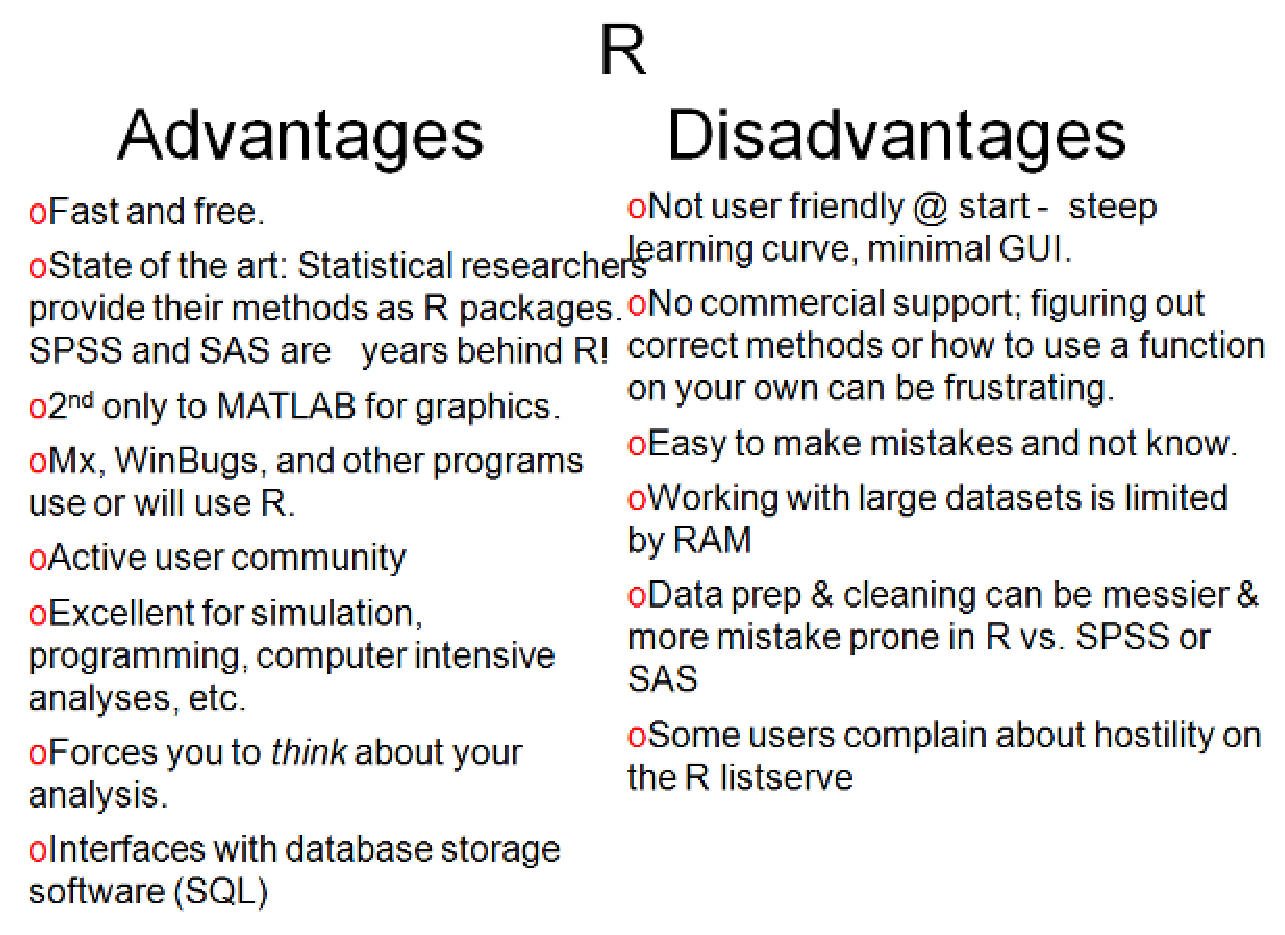
\includegraphics[height=7cm]{./images/R_strong_weak.eps}}
    \caption{Analyze R language}\label{fig:R_strong_weak}
  \end{figure}


\section{Comparison with other tools}
\label{sec:comp-with-other}


\begin{figure}[htb]
    \centerline{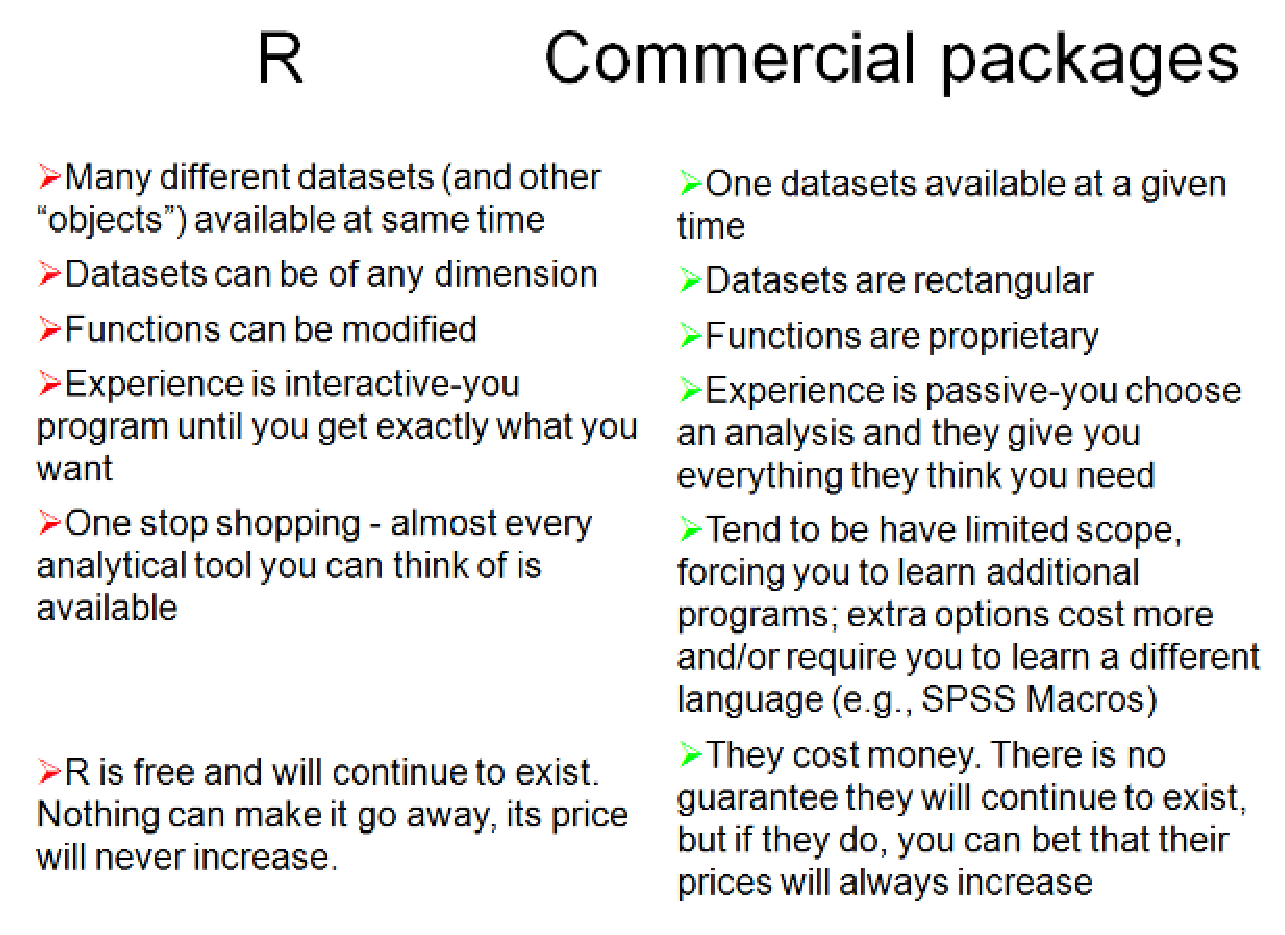
\includegraphics[height=7cm]{./images/R_others.eps}}
    \caption{Compare R language and other commercial softwares}\label{fig:R_others}
  \end{figure}


\begin{figure}[htb]
    \centerline{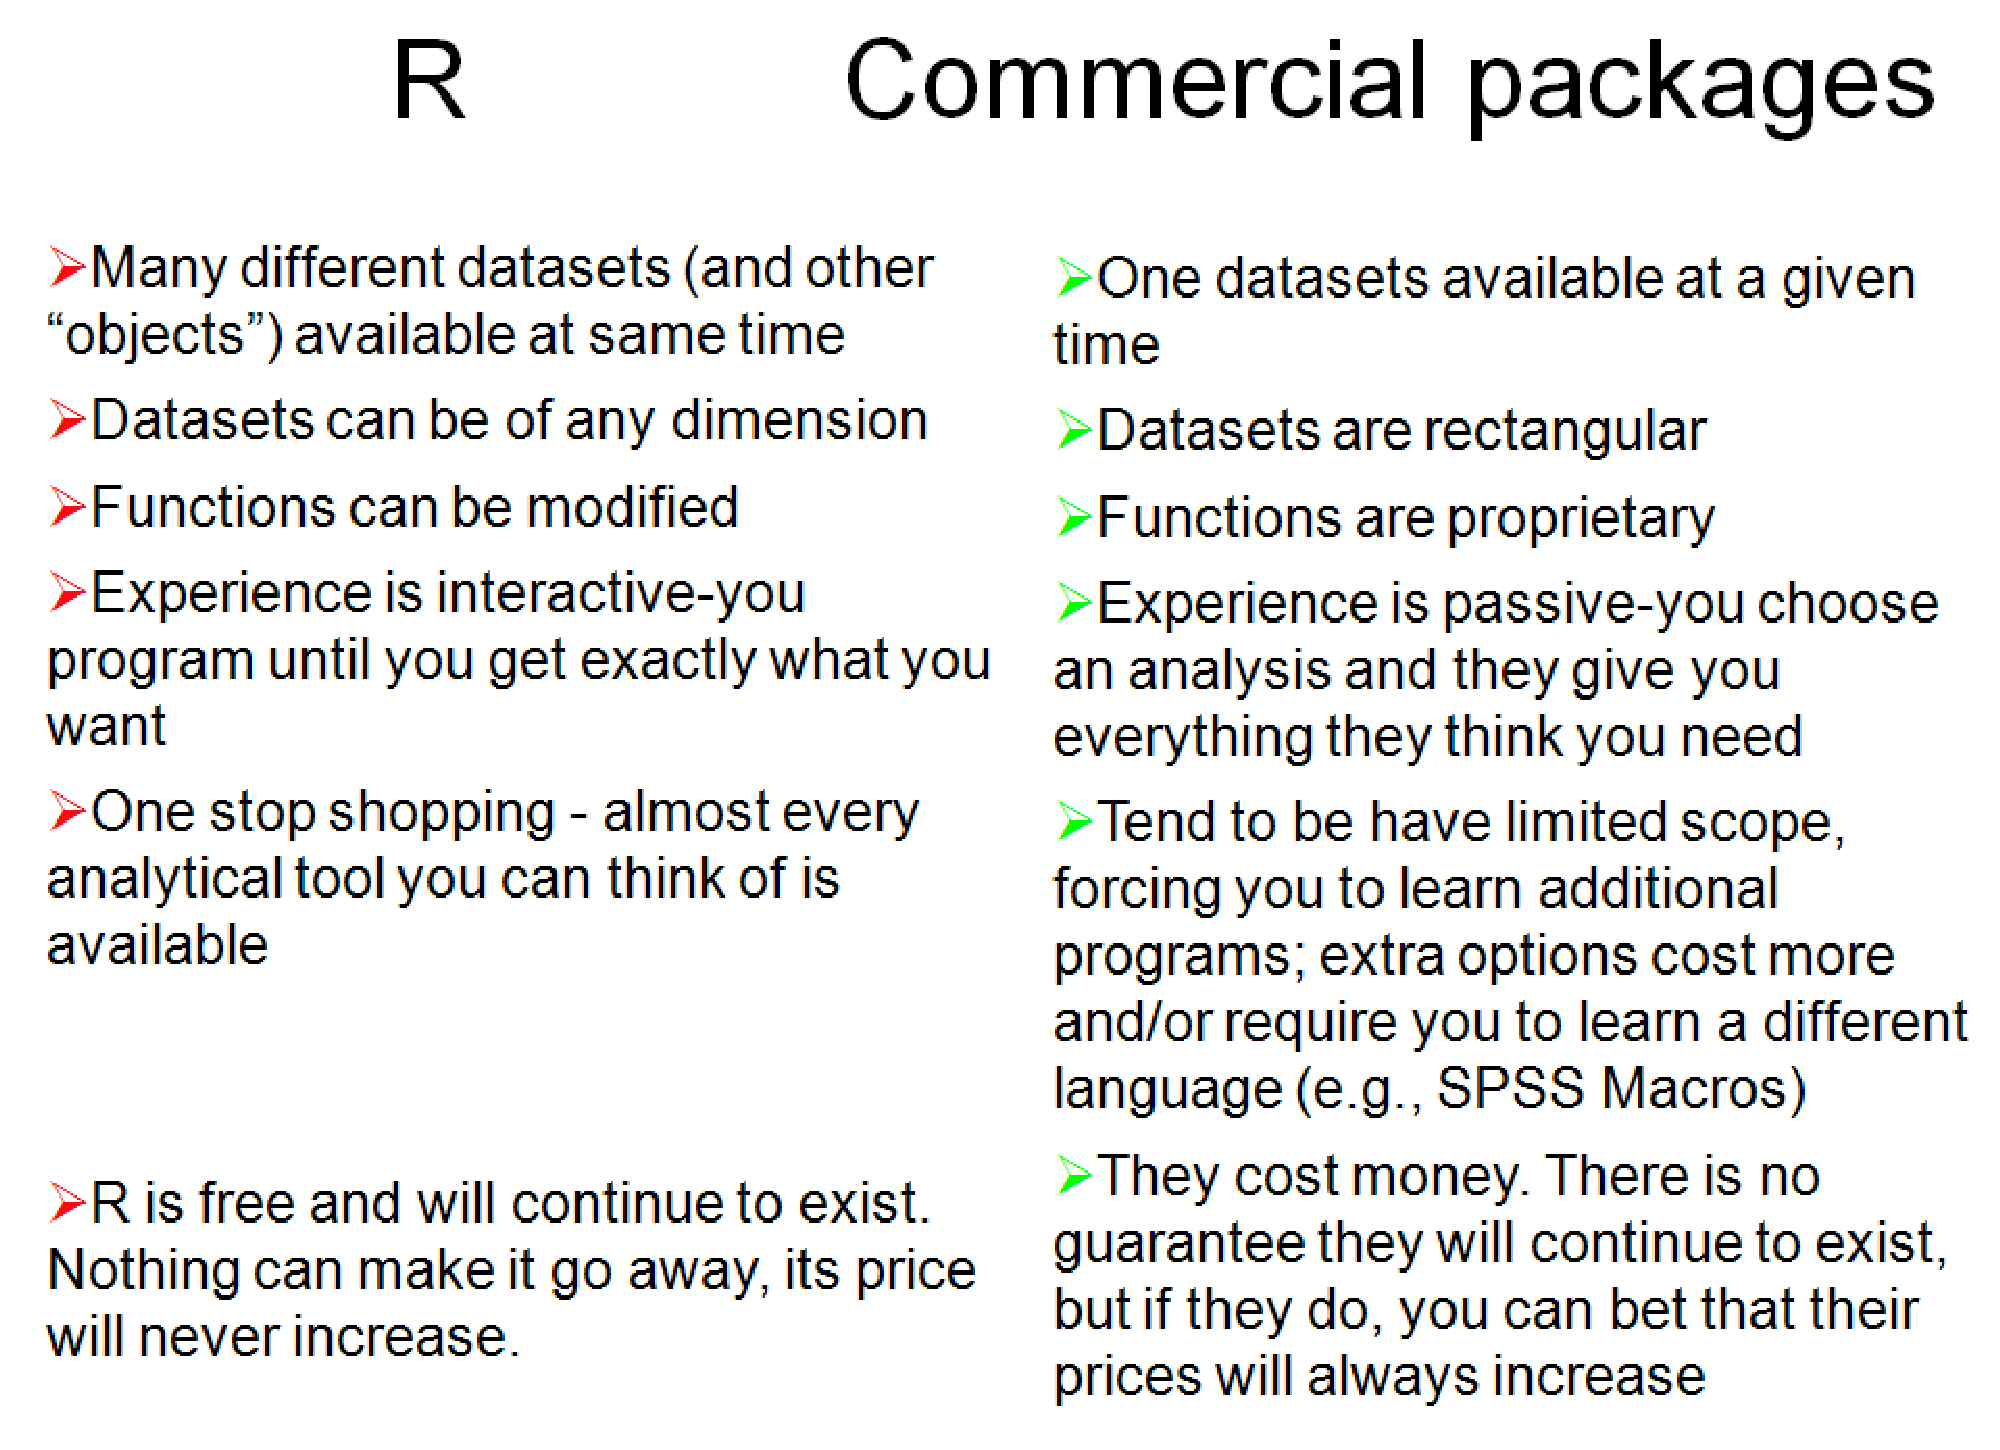
\includegraphics[height=7cm]{./images/R_SPSS_1.eps}}
    \caption{Compare R language and SAS/SPSS}\label{fig:R_SPSS_1}
\end{figure}
\begin{figure}[htb]
  \centerline{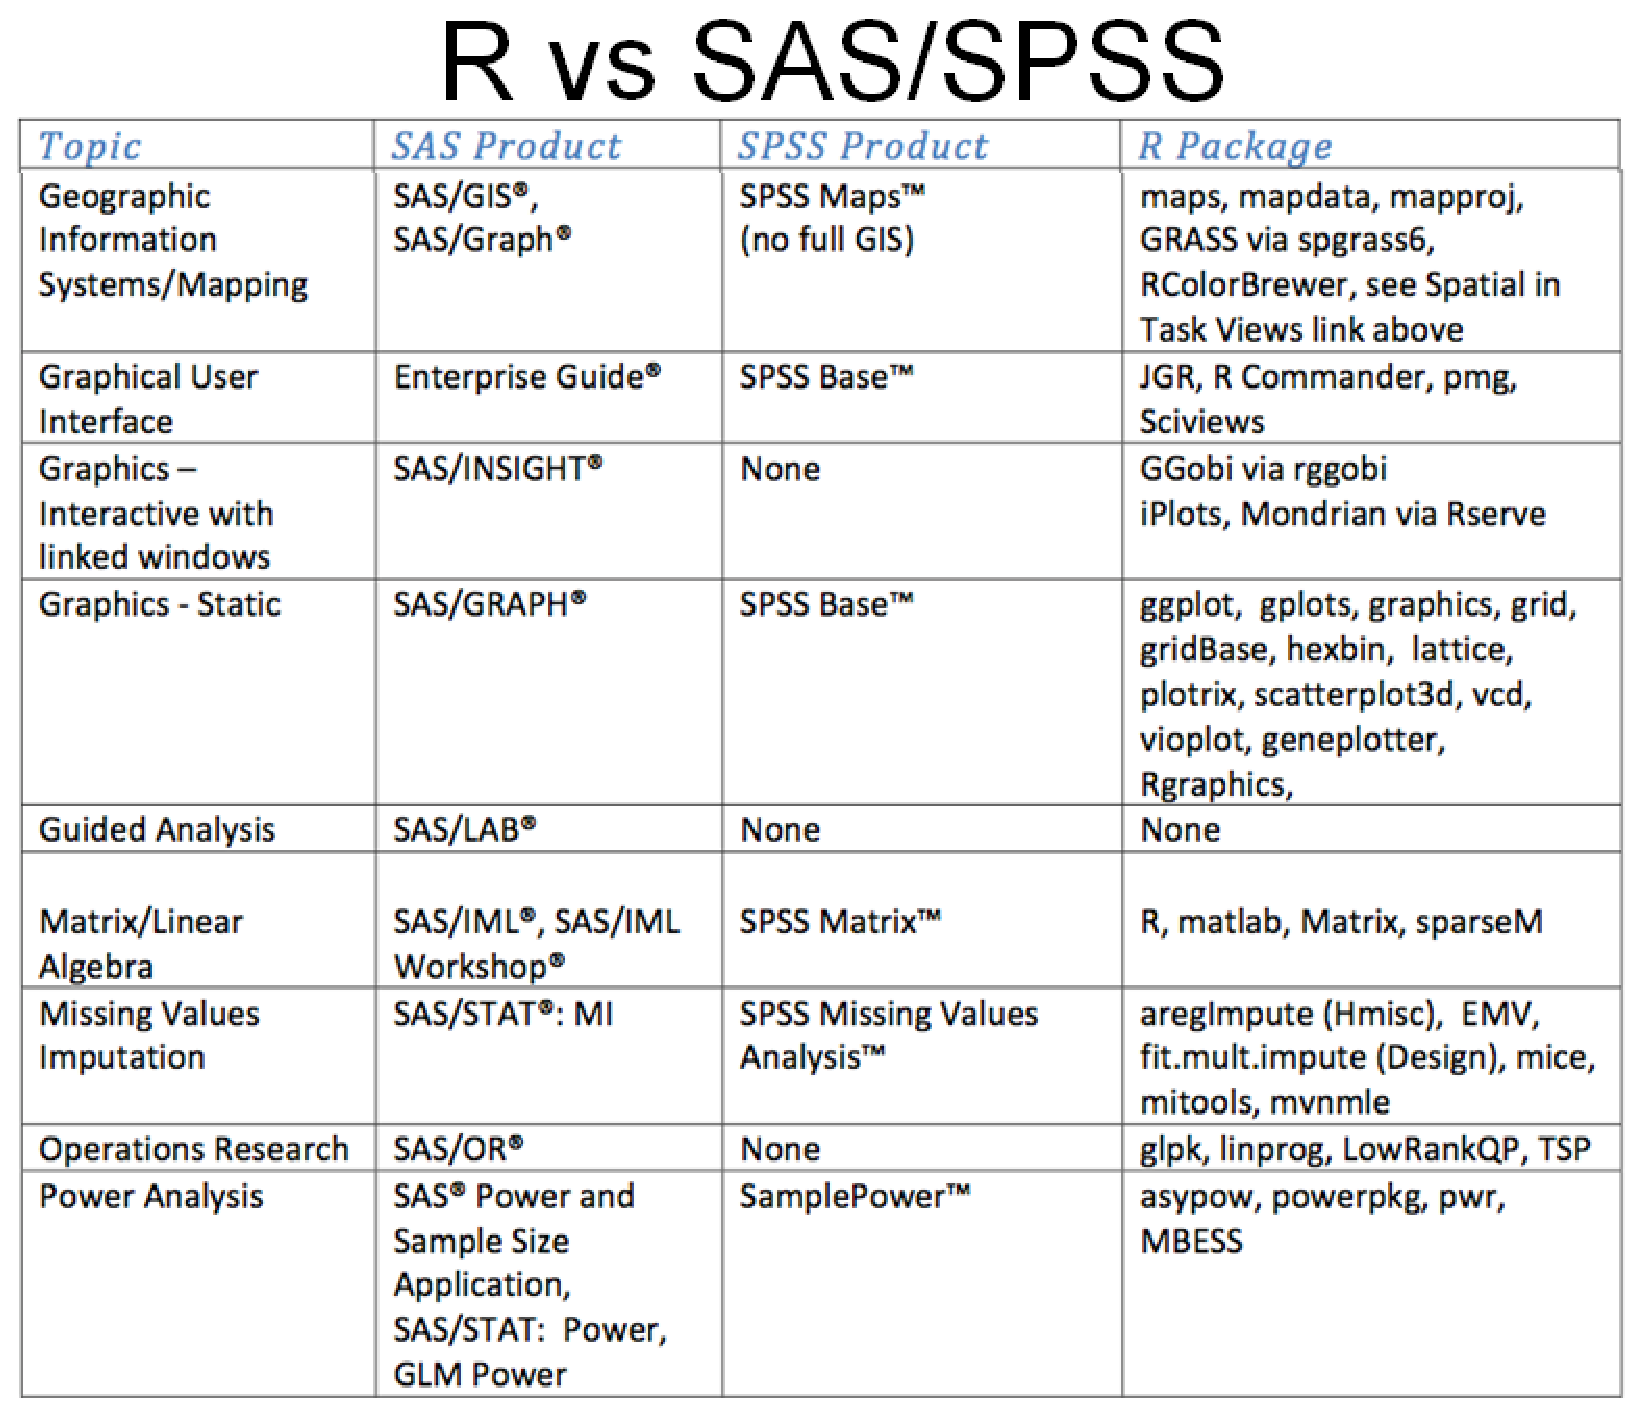
\includegraphics[height=7cm]{./images/R_SPSS_2.eps}}
  \caption{Compare R language and SAS/SPSS}\label{fig:R_SPSS_2}
\end{figure}
\begin{figure}[htb]
  \centerline{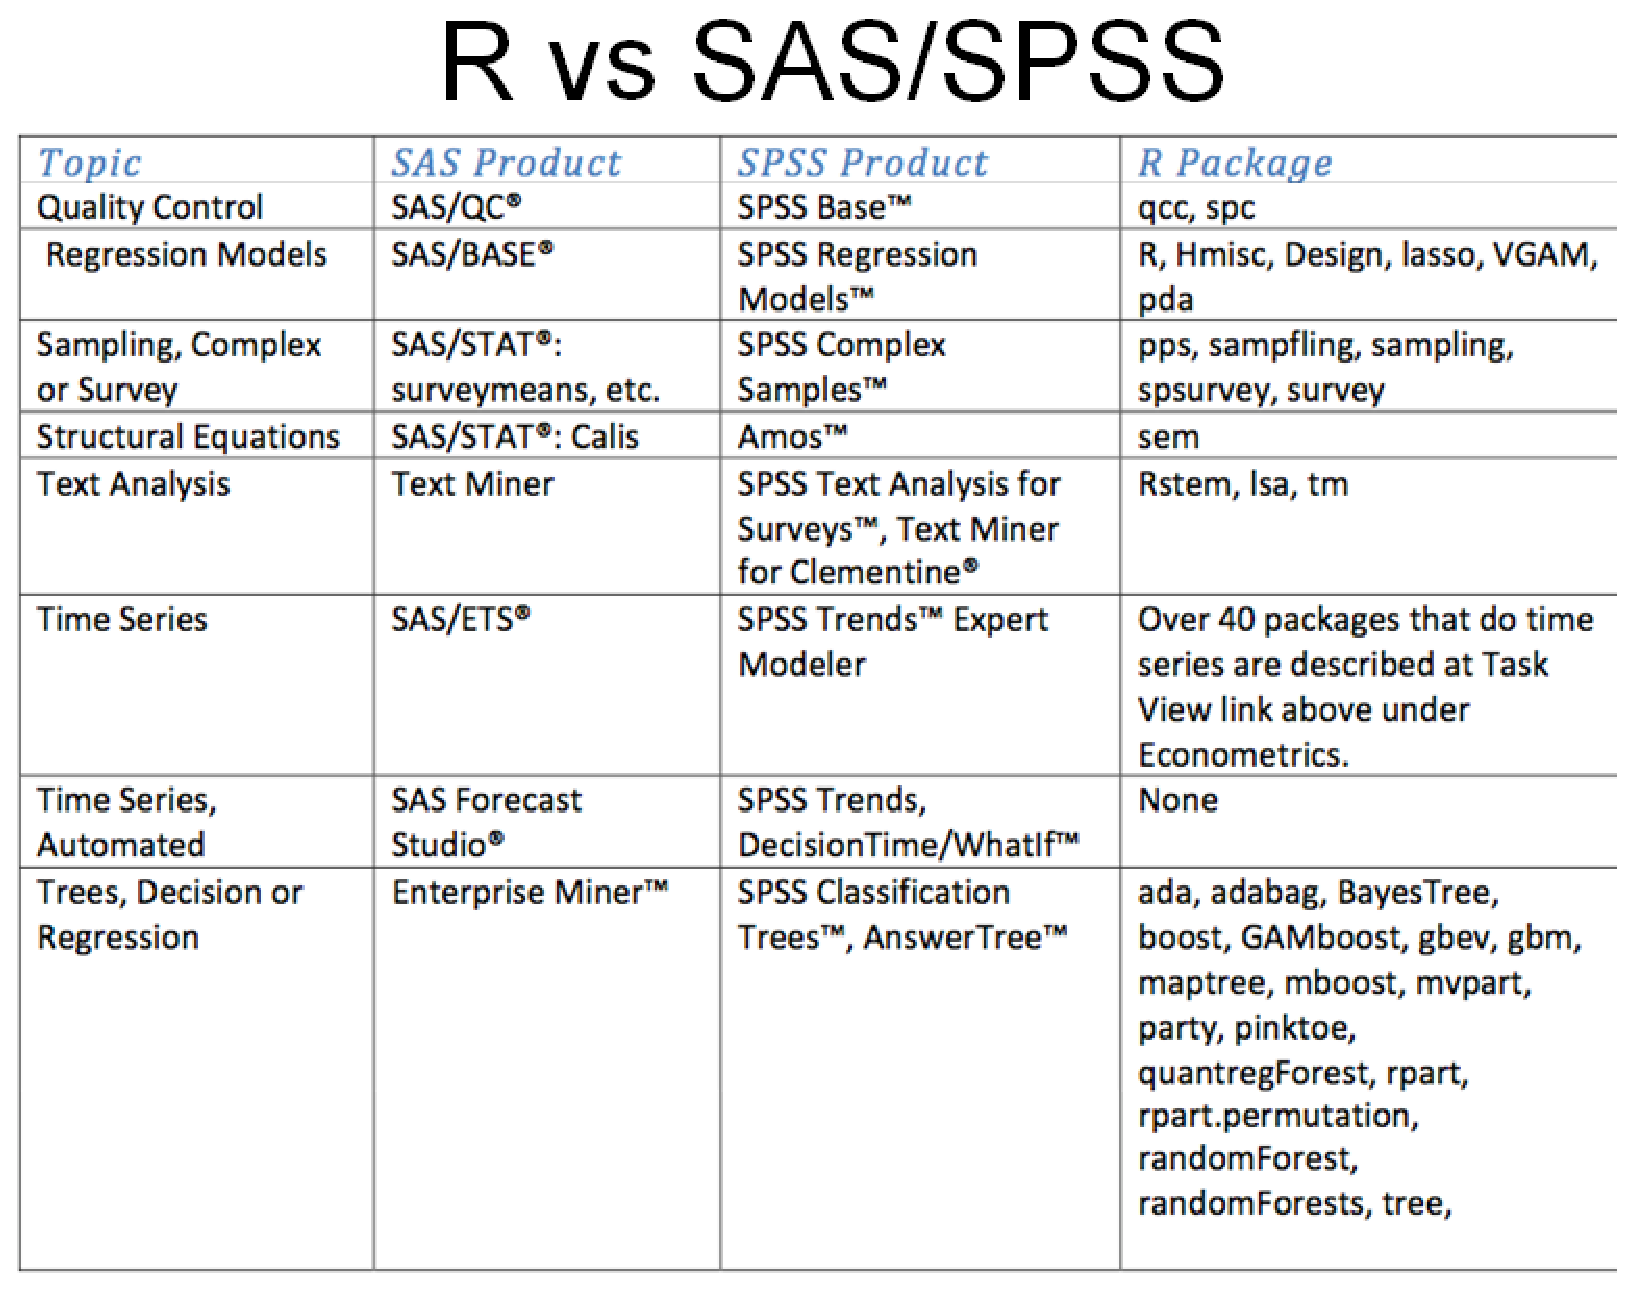
\includegraphics[height=7cm]{./images/R_SPSS_3.eps}}
  \caption{Compare R language and SAS/SPSS}\label{fig:R_SPSS_3}
\end{figure}


\section{Workspace}
\label{sec:workspace}

{\bf Namespace} is an abstract concept that hold items (variables,
objects, classes...). This is a common notion in C/C++ and some other
programming language. As a rule, names in a namespace cannot have more
than one meaning, i.e. two different items cannot have the same
name. In R, everything is put into a root namespace, called
{\bf workspace} (root working environment, global environment).

When you open R interpreter, a workspace is created. Everything you
create (variables, functions…) are stored in this workspace (workspace
acts like a directory, while variables, functions act like files). 
The namespaces of lower levels are {\it lexical environments} (scope), e.g. every
call to a function create a new evaluation frame with a lexical (local)
environment, or context created internally in the {\it call
  stack}. When a function has finished evaluating, its context is
removed from the call stack.

Here are some commands to deal with things in a workspace:
\begin{itemize}
\item To get the list of names (e.g. objects, user-defined
  functions) currently defined in this workspace, use {\bf ls()}
  or {\bf objects()} command.  
\begin{lstlisting}
>>  ls ()
>>  objects()
\end{lstlisting}

\item To remove a name from the workspace, use {\bf rm()} or {\bf
    remove()} command
\begin{lstlisting}
 >> rm (name1 [,name2]) # where name(s) can be any
         # defined objects or user-defined functions
\end{lstlisting}

\item To remove objects whose names are given in a list, you can pass
  the list to the parameter {\it list} or the {bf rm()} command,
  e.g. remove all objects or user-defined functions from the workspace

\begin{lstlisting}
        # be careful : all lower cases
>> rm (list = ls()) 
\end{lstlisting}

\item The current workspace can be saved for later use. Before you
  exit the R interpreter, you use the menu bar (File\verb|->|save workspace),
  or from the command line:
\begin{lstlisting}
>> save(name1 [, name2], file="Filename.Rdata")  # save some names only
>> save.image()           # save the whole workspace to 
      # the default file ".Rdata" in the current working directory
>> save.image(file="Filename.Rdata")
\end{lstlisting}
  where {\it name} can be any object names or user-defined
  functions

\item To save, load, or display the command line history 
\begin{lstlisting}
>> savehistory() # save to default ".Rhistory" file
>  savehistory(file="MyData.Rhistory") 
>  loadhistory(file="MyData.Rhistory") 
>  history()      # display last 25 commands
>  history(max.show=Inf) # display all commands
\end{lstlisting}

\end{itemize}

Access to the call stack is provided through a family of functions
which have names that start with 'sys.'. They are listed briefly
below.

\begin{verbatim}
sys.call
   Get the call for the specified context. 
sys.frame
   Get the evaluation frame for the specified context. 
sys.nframe
   Get the environment frame for all active contexts. 
sys.function
   Get the function being invoked in the specified context. 
sys.parent
   Get the parent of the current function invocation. 
sys.calls
   Get the calls for all the active contexts. 
sys.frames
   Get the evaluation frames for all the active contexts. 
sys.parents
   Get the numeric labels for all active contexts. 
sys.on.exit
   Set a function to be executed when the 
   specified context is exited.   
sys.status
   Calls sys.frames, sys.parents and sys.calls. 
parent.frame
   Get the evaluation frame for the specified parent context.
\end{verbatim}

\section{Getting Helps}
\label{sec:getting-helps}

Why we need help? 

\begin{itemize}
\item To have a brief view of R, we can use
\begin{lstlisting}
>> help.start()
\end{lstlisting}
  launch a web browser which shows 2 important sections:
  {\it An introduction to R} (lots of examples, tips, \& explanation),
  {\it Packages} (which has the {\bf Base} package that contains
  everything for a novice, {\bf stat} package for statistical
  functions and {\bf graphics} packages for common graphical
  visualization routines)

\item We know that functions are organized into packages. To see all
  installed packages. NOTE: not all of them are loaded in the session
\begin{lstlisting}
>>library()	
\end{lstlisting}

\item In order to use functions provided by a package, you need to
  load that package, use either {\bf library()} or {\bf require()}
  commands
\begin{lstlisting}
>> library(libName1 [,libName2])
>> require(libName)   # designed to used inside function calls
\end{lstlisting}
  with {\it libName} is the name any of the packages listed when you call
  {\bf library()}.

\item To see which packages have been loaded, you can use
  {\bf search()} command
\begin{lstlisting}
>> search()   
[1] ".GlobalEnv"    "...:stats" "...:graphics" 
[4] "...:grDevices" "...:utils" "...:datasets" 
[7] "...:methods"   "Autoloads" "package:base"     
 # to fit the page margin: "package" 
 # has been replaced by ...
\end{lstlisting}
  Each one with an indexed value.  

\item List all functions within a loaded package
\begin{lstlisting}
>> ls(pos=idx) 
\end{lstlisting}
  where {\it idx} is the index of the package found in the
  {\bf search()} command, the first index (idx=1) is always the
  {\bf .GlobalEnv}.

\item Look for function name and its meaning
\begin{lstlisting}
>> help(func_name)
>> help.search('part_of_func_name')
>> help.search("part_of_func_name")
>> ? func_name
\end{lstlisting}

\item If you don't remember the full function or object's name, you can use the
  {\bf appropos()} or {\bf find()} command
\begin{lstlisting}
>> apropos("what", where = FALSE, 
        ignore.case = TRUE, mode = "any")  
\end{lstlisting}
  return a vector of which the elements are the names of all functions
  or objects whose partial name is matching with {\it what}. To
  restrict the search, we can explicitly tell the
  \hyperref[mode]{mode}.

\begin{lstlisting}
>> find(what, mode = "any", numeric = FALSE, 
             simple.words = TRUE)
\end{lstlisting}
return a vector of which the elements are the names of all packages
matching with {\it what}. By default, {\it what} must be a complete
word in the package name; otherwise, we use {\it simple.words=FALSE}.

\item To pause/interrupt the execution, normally inside a function, so
  that user can inspect the values of objects, use the {\bf browser()}
  command
\begin{lstlisting}
>> browser()
\end{lstlisting}
Then, to continue the execution, just press {\bf c} and enter.
\end{itemize}

\subsection{Scopes}
\label{sec:scopes}

In any programming language, to allow different objects of the same
names, they are held in different abstract holders called
{\it namespace}. In addition, an object defined within a function
cannot be used out of it. We call this the scope of an object.  In the
code, whenever a symbolic name occurs, its value will be accessed by a
process called {\it scoping}, an internal search for the value of that
symbol.

In the body of a function, variables are either supplied through the
formal argument list, local variables (both are bound) or unbound
(=free). 
\begin{lstlisting}
a <- 1
f <- function() { a <- 2; a }
print (a) # 1, => a does not change, then a is unbound
\end{lstlisting}

Any variable appearing in the function body is first searched for in
the function's {\it evaluation environment}, then in its
{\it definition environment} (which has become the parent environment
({\bf enclosure}) of the former by the call of the function) and so on
up to the {\it global environment} (=root of the workspace), then
along the search path of environments until the {\it base
  package}.

(In R everything lives in (possibly nested) environments, which are a
nesting of frames (=set of local variables created in a
function). search() shows the search path.) Bound variables are
already found on the lowest level; supplied arguments are practically
treated as local. Unbound variables are not found on the lowest
level. The mentioned nesting of the evaluation environment in the
definition environment makes R's scoping lexical: The value of an
unbound variable is essentially determined by the bindings that were
in effect at the time of the creation of the function. In contrast,
with static scoping as in S, it is determined on the global
environment level. (Dynamic scoping lets it be determined by the most
recent (in time) definition, jumping up the call stack


\subsection{Generic}
\label{sec:generic}

Multiline (multi-line) statement in R is very special. You don't have
to use any special symbol to denote a multiline statement, e.g. in
2Matlab you have to specify ... at the end of the line. R statistic
automatically detect the multiline statement. However, make sure that
the operator in an expression should be on the preceding line.

Example:
\begin{lstlisting}
  4 + 4 + 
     1
\end{lstlisting}
is 9, but
\begin{lstlisting}
  4 + 4 
    + 1
\end{lstlisting}
is 8.


\subsection{Control statements}
\label{sec:control-statements}

Here, we discuss control statements:

\subsubsection{Grouped expressions}
\label{sec:grouped-expressions}

\verb!{expression_1; expression_2; …}!  
\begin{itemize}
\item return the last expression evaluated
\item similar to compound statements in C
\end{itemize}

\subsubsection{Conditions}
\label{sec:conditions}

\verb!if (…) else {…}!
\begin{verbatim}
if (expression_1) expr_2 else expr_3
\end{verbatim}
expression\_1 should return a logical value, operator \verb!||! and
\&\& may be used

\subsubsection{Test}
\label{sec:test}


\begin{lstlisting}
ifelse(test, do_yes, do_no)
\end{lstlisting}
which call \verb|do_yes| if test is TRUE, and call \verb|do_no|
otherwise.

\subsubsection{Finite loops}
\label{sec:finite-loops}

{\bf for} loops: 
\begin{verbatim}
for (name in expr_1) expr_2
\end{verbatim}

\begin{itemize}
\item name is the loop variable
\item expr\_1 is often a sequence, created by using seq() function or
  using start:end structure
\end{itemize}

\subsubsection{Infinite loops}
\label{sec:infinite-loops}


{\bf repeat} loops: 
\begin{verbatim}
repeat expr
\end{verbatim}

\begin{itemize}
\item continually evaluate expr
\item loop must be terminated using break;
\end{itemize}

{\bf while} loops:
\begin{verbatim}

while (expr_1) expr_2
\end{verbatim}

\begin{itemize}
\item while expr\_1 is FALSE, evaluate expr\_2
\item to manipulate the loop, the break; and next; statement can be
  used
\end{itemize}

\subsubsection{Next, break}
\label{sec:next-break}

 {\it next, break} statements

\begin{lstlisting}
muy = 120
sigma = 24

n = 100
x = matrix(0, nrow = n, ncol = n)
for (i in 1:n) {
  set.seed(i)
  x[i,] = rnorm(100, mean = muy, sd = sigma)
}
\end{lstlisting}

\subsection{Functions}
\label{sec:functions}

\subsection{Packages}
\label{sec:packages}

Each package may come with a set of examples (demos), we can run the
these example, to demonstrate for the usage of a particular function,
using example() function.
\begin{lstlisting}
         # get the examples on how to use a function
>> example(func_name)	
\end{lstlisting}

\section{Technical terms}
\label{sec:technical-terms}

What {\bf proportion} of men in this age group have smoked for more
than 20 years? - (i.e. what is the probability) we need to define a
r.v. X expressing the duration of smoking time for men.

What {\bf percentage} of values would fall in this range? - (i.e. what
is the probability). 


\section{Data format in R}


\subsection{data.frame}
\label{sec:data.frame-intro}


A more details of data.frame is given in Sect.\ref{sec:data.frame}.

The traditional R-based functions
\begin{verbatim}

read.table()

read.delim()

read.csv()
\end{verbatim}
import data into R as a \verb!data.frame!.


Create a data.frame
\begin{verbatim}

# create a dataframe with 4 fields
friends_data <- data.frame(name = my_friends,
         age = friend_ages,
         height = c(180, 170, 120),
         married = are_married
        )
        
        
# convert from matrix
# NOTE: t(.) can be used to transpose a matrix
class(my_data)
# --> "matrix"

my_df <- as.data.frame(my_data)
    
        
# check type
is.data.frame(friends_data)

is.data.frame(my_data)
\end{verbatim}

\subsection{-- indexing columns}


Use fieldname after \verb!$!
\begin{verbatim}
data_frame$name

# or

data_frame[, "name"]

# or a few columns using indices, or names
data_frame[, c(1, 4)]
data_frame[, c("name", "age")]


# exclude a column by using negative index

data_frame[, -1]
\end{verbatim}


\subsection{-- select rows}

Select rows in that column's data matching condition
\begin{verbatim}

# true, or false list
data_frame$age >= 27

# we can use above list of true, false to retrieve rows
data_frame[ data_frame$age >= 27, ]

data_frame[ data_frame$age >= 27, c(1, 2)]

\end{verbatim}

\subsection{-- extend/add columns}

Add a new column 
\begin{verbatim}
data_frame$new_column_name <- friends_groups
\end{verbatim}

\subsection{tibble}
\label{sec:tibble-intro}

The most modern R package \verb!readr! provides several fast functions, better
than R-based functions.
These functions import data as a \verb!tbl_df! (pronounced: tibble diff), which
is better when working with large data sets.

Tibble is a modern rethinking of R's data.frame (Sect.\ref{sec:data.frame}).

\section{R-studio (RStudio)}


\subsection{Issue after updating Java}

Issue
\begin{verbatim}
> library(rJava)
Error: package or namespace load failed for 'rJava':
 .onLoad failed in loadNamespace() for 'rJava', details:
  call: dyn.load(file, DLLpath = DLLpath, ...)
  error: unable to load shared object '/Users/kevin/Library/R/3.4/library/rJava/libs/rJava.so':
  dlopen(/Users/kevin/Library/R/3.4/library/rJava/libs/rJava.so, 6): Library not loaded: @rpath/libjvm.dylib
  Referenced from: /Users/kevin/Library/R/3.4/library/rJava/libs/rJava.so
  Reason: image not found
\end{verbatim}


\url{https://github.com/rstudio/rstudio/issues/2254}

SOLUTION: That typically needs to be run after an update of the system Java installation
\begin{verbatim}
sudo R CMD javareconf
\end{verbatim}

\subsection{Issue with memory}

\url{https://stackoverflow.com/questions/51295402/r-on-macos-error-vector-memory-exhausted-limit-reached}

\begin{verbatim}
Error: vector memory exhausted (limit reached?)
\end{verbatim}

NOTE
\begin{verbatim}
Sys.setenv('R_MAX_VSIZE'=32000000000)
\end{verbatim}
, as has been suggested on multiple StackOverflow posts, only works on the
command line, and that setting that parameter while using Rstudio does not
prevent this error:

\begin{verbatim}
• The environment variable R_MAX_VSIZE can now be used to specify 
       the maximal vector heap size. On macOS, unless specified by this 
       environment variable, the maximal vector heap size is set to the 
       maximum of 16GB and the available physical memory. This is to 
       avoid having the R process killed when macOS over-commits memory. 
       
You can set R_MAX_VSIZE to a larger value but you should do some 
experimenting to decide on a safe value for your system. Mac OS is 
quite good at using virtual memory up to a point but then gets very bad
\end{verbatim}

SOLUTION:
\begin{verbatim}
cd ~
touch .Renviron
open .Renviron

R_MAX_VSIZE=100Gb 
\end{verbatim}
This limit includes both physical and virtual memory
\subsection{O/S specific: Mac O/S, Windows, Linux}


\begin{verbatim}
> .Platform
$OS.type
[1] "unix"

$file.sep
[1] "/"

$dynlib.ext
[1] ".so"

$GUI
[1] "RStudio"

$endian
[1] "little"

$pkgType
[1] "mac.binary.el-capitan"

$path.sep
[1] ":"

$r_arch
[1] ""

\end{verbatim}

Example:
\begin{verbatim}
if(.Platform$OS.type == "windows") withAutoprint({
memory.size()
memory.size(TRUE)
memory.limit()
})
\end{verbatim}

\subsection{Options}
\label{sec:options}

There are various global options that you can adjust to fit your
needs. Use {\bf options()} command with no arguments to display the
list of available options. 

\subsection{-- set maximum memory for alloc() }

\begin{verbatim}
# call this before loading any packages

options(java.parameters = "-Xmx4024m")
\end{verbatim}


\subsection{pass data by reference?}

\url{https://stackoverflow.com/questions/2603184/can-you-pass-by-reference-in-r}



\section{R notebook}


To use a package
\begin{verbatim}
```{r}

# install a package
install.packages("tibble")


# use it
library("tibble")
```
\end{verbatim}


%%% Local Variables: 
%%% mode: latex
%%% TeX-master: "R_language"
%%% End: 
